\documentclass{standalone}
\usepackage{tikz}
\usetikzlibrary{patterns, positioning}
\usepackage[sfdefault]{ClearSans} %% option 'sfdefault' activates Clear Sans as the default text font
\usepackage[T1]{fontenc}

\begin{document}
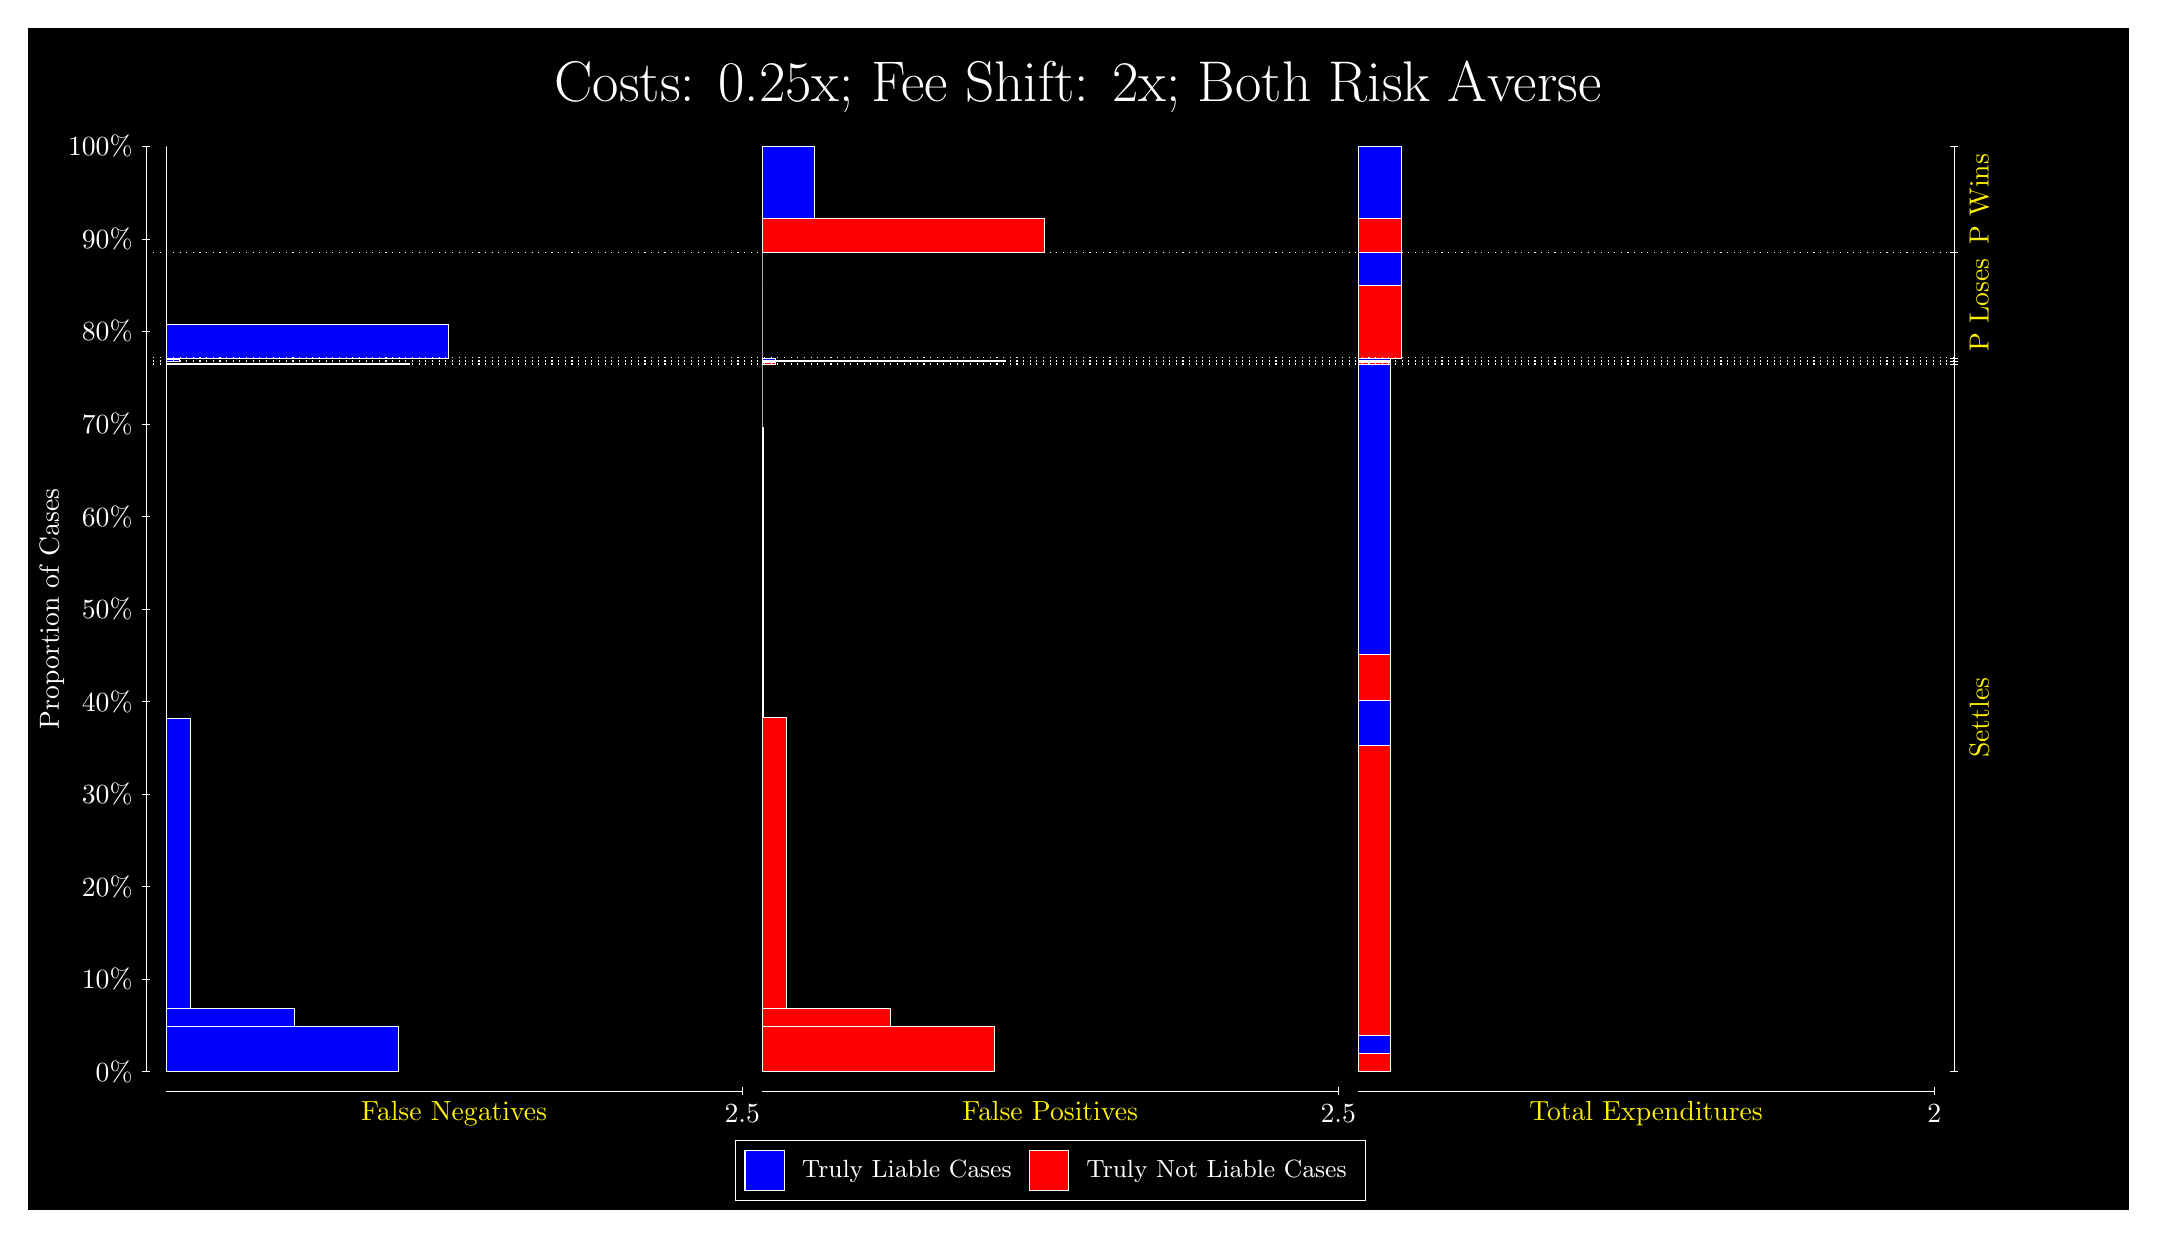
\begin{tikzpicture}
\draw[fill=black] (0,0) rectangle (26.667,15);
\draw[text=white] (0,13.5) rectangle (26.667,15) node[midway] {\huge Costs: 0.25x; Fee Shift: 2x; Both Risk Averse};
\draw[white, very thin] (1.5,1.75) -- (1.5,13.5);
\node[rotate=90, text=white, anchor=center] at (0.3, 7.625) {Proportion of Cases};
\draw[white, very thin] (1.45,1.75) -- (1.55,1.75);
\node[text=white, anchor=east] at (1.45, 1.75) {0\%};
\draw[white, very thin] (1.45,2.925) -- (1.55,2.925);
\node[text=white, anchor=east] at (1.45, 2.925) {10\%};
\draw[white, very thin] (1.45,4.1) -- (1.55,4.1);
\node[text=white, anchor=east] at (1.45, 4.1) {20\%};
\draw[white, very thin] (1.45,5.275) -- (1.55,5.275);
\node[text=white, anchor=east] at (1.45, 5.275) {30\%};
\draw[white, very thin] (1.45,6.45) -- (1.55,6.45);
\node[text=white, anchor=east] at (1.45, 6.45) {40\%};
\draw[white, very thin] (1.45,7.625) -- (1.55,7.625);
\node[text=white, anchor=east] at (1.45, 7.625) {50\%};
\draw[white, very thin] (1.45,8.8) -- (1.55,8.8);
\node[text=white, anchor=east] at (1.45, 8.8) {60\%};
\draw[white, very thin] (1.45,9.975) -- (1.55,9.975);
\node[text=white, anchor=east] at (1.45, 9.975) {70\%};
\draw[white, very thin] (1.45,11.15) -- (1.55,11.15);
\node[text=white, anchor=east] at (1.45, 11.15) {80\%};
\draw[white, very thin] (1.45,12.325) -- (1.55,12.325);
\node[text=white, anchor=east] at (1.45, 12.325) {90\%};
\draw[white, very thin] (1.45,13.5) -- (1.55,13.5);
\node[text=white, anchor=east] at (1.45, 13.5) {100\%};

\draw[white, very thin] (24.457,1.75) -- (24.457,13.5);
\draw[white, very thin] (24.407,1.75) -- (24.507,1.75);
\node[anchor=west] at (24.407, 1.75) {};
\draw[white, very thin] (24.407,10.735) -- (24.507,10.735);
\node[anchor=west] at (24.407, 10.735) {};
\draw[white, very thin] (24.407,10.774) -- (24.507,10.774);
\node[anchor=west] at (24.407, 10.774) {};
\draw[white, very thin] (24.407,10.813) -- (24.507,10.813);
\node[anchor=west] at (24.407, 10.813) {};
\draw[white, very thin] (24.407,12.156) -- (24.507,12.156);
\node[anchor=west] at (24.407, 12.156) {};
\draw[white, very thin] (24.407,13.5) -- (24.507,13.5);
\node[anchor=west] at (24.407, 13.5) {};

\draw[white, very thin, fill=blue] (1.75,1.75) rectangle (4.6958,2.323);
\draw[white, very thin, fill=blue] (1.75,2.323) rectangle (3.3784,2.5504);
\draw[white, very thin, fill=blue] (1.75,2.5504) rectangle (2.0611,6.2425);
\draw[white, very thin, fill=red] (1.75,6.2425) rectangle (1.75,10.735);
\draw[white, very thin, fill=blue] (1.75,10.735) rectangle (4.8422,10.747);
\draw[white, very thin, fill=red] (1.75,10.747) rectangle (1.75,10.774);
\draw[white, very thin, fill=blue] (1.75,10.774) rectangle (1.9147,10.801);
\draw[white, very thin, fill=red] (1.75,10.801) rectangle (1.75,10.813);
\draw[white, very thin, fill=blue] (1.75,10.813) rectangle (5.3362,11.237);
\draw[white, very thin, fill=red] (1.75,11.237) rectangle (1.75,12.156);
\draw[white, very thin, fill=red] (1.75,12.156) rectangle (1.75,12.58);
\draw[white, very thin, fill=blue] (1.75,12.58) rectangle (1.75,13.5);
\draw[white, very thin, fill=red] (9.3189,1.75) rectangle (12.265,2.323);
\draw[white, very thin, fill=red] (9.3189,2.323) rectangle (10.947,2.5504);
\draw[white, very thin, fill=red] (9.3189,2.5504) rectangle (9.6299,6.2427);
\draw[white, very thin, fill=blue] (9.3189,6.2427) rectangle (9.3372,9.9348);
\draw[white, very thin, fill=blue] (9.3189,9.9348) rectangle (9.3189,10.735);
\draw[white, very thin, fill=red] (9.3189,10.735) rectangle (9.4835,10.762);
\draw[white, very thin, fill=blue] (9.3189,10.762) rectangle (9.3189,10.774);
\draw[white, very thin, fill=red] (9.3189,10.774) rectangle (12.411,10.786);
\draw[white, very thin, fill=blue] (9.3189,10.786) rectangle (9.4835,10.813);
\draw[white, very thin, fill=red] (9.3189,10.813) rectangle (9.3189,11.732);
\draw[white, very thin, fill=blue] (9.3189,11.732) rectangle (9.3189,12.156);
\draw[white, very thin, fill=red] (9.3189,12.156) rectangle (12.905,12.58);
\draw[white, very thin, fill=blue] (9.3189,12.58) rectangle (9.9776,13.5);
\draw[white, very thin, fill=red] (16.888,1.75) rectangle (17.299,1.9774);
\draw[white, very thin, fill=blue] (16.888,1.9774) rectangle (17.299,2.2048);
\draw[white, very thin, fill=red] (16.888,2.2048) rectangle (17.299,5.8971);
\draw[white, very thin, fill=blue] (16.888,5.8971) rectangle (17.299,6.4701);
\draw[white, very thin, fill=red] (16.888,6.4701) rectangle (17.299,7.0431);
\draw[white, very thin, fill=blue] (16.888,7.0431) rectangle (17.299,10.735);
\draw[white, very thin, fill=red] (16.888,10.735) rectangle (17.299,10.762);
\draw[white, very thin, fill=blue] (16.888,10.762) rectangle (17.299,10.774);
\draw[white, very thin, fill=red] (16.888,10.774) rectangle (17.299,10.786);
\draw[white, very thin, fill=blue] (16.888,10.786) rectangle (17.299,10.813);
\draw[white, very thin, fill=red] (16.888,10.813) rectangle (17.437,11.732);
\draw[white, very thin, fill=blue] (16.888,11.732) rectangle (17.437,12.156);
\draw[white, very thin, fill=red] (16.888,12.156) rectangle (17.437,12.58);
\draw[white, very thin, fill=blue] (16.888,12.58) rectangle (17.437,13.5);
\draw[white, dotted] (1.5,10.735) -- (24.457,10.735);
\draw[white, dotted] (1.5,10.774) -- (24.457,10.774);
\draw[white, dotted] (1.5,10.813) -- (24.457,10.813);
\draw[white, dotted] (1.5,12.156) -- (24.457,12.156);
\draw[white, very thin] (1.75,1.5) -- (9.0689,1.5);
\node[text=yellow, anchor=north] at (5.4094, 1.5) {False Negatives};
\draw[white, very thin] (9.0689,1.45) -- (9.0689,1.55);
\node[text=white, anchor=north] at (9.0689, 1.45) {2.5};

\draw[white, very thin] (9.3189,1.5) -- (16.638,1.5);
\node[text=yellow, anchor=north] at (12.978, 1.5) {False Positives};
\draw[white, very thin] (16.638,1.45) -- (16.638,1.55);
\node[text=white, anchor=north] at (16.638, 1.45) {2.5};

\draw[white, very thin] (16.888,1.5) -- (24.207,1.5);
\node[text=yellow, anchor=north] at (20.547, 1.5) {Total Expenditures};
\draw[white, very thin] (24.207,1.45) -- (24.207,1.55);
\node[text=white, anchor=north] at (24.207, 1.45) {2};

\node[text=yellow, centered, rotate=90] at (24.777, 6.2426) {Settles};


\node[text=yellow, centered, rotate=90] at (24.777, 11.485) {P Loses};
\node[text=yellow, centered, rotate=90] at (24.777, 12.828) {P Wins};

\draw (12.978300999999998,1.5) node[draw=none] (baseCoordinate) {};
\begin{scope}[align=center]
        \matrix[scale=0.5, draw=white, below=0.5cm of baseCoordinate, nodes={draw}, column sep=0.1cm]{
            \node[rectangle, draw, minimum width=0.5cm, minimum height=0.5cm, fill=blue] {}; &
            \node[draw=none, font=\small, text=white] (B) {Truly Liable Cases}; &
            \node[rectangle, draw, minimum width=0.5cm, minimum height=0.5cm, fill=red] {}; &
            \node[draw=none, font=\small, text=white] (B) {Truly Not Liable Cases}; \\
            };
\end{scope}

\end{tikzpicture}
\end{document}